\section{Principal Component Analysis}
\label{PCA}
La \textbf{P}rincipal \textbf{C}omponent \textbf{A}nalysis (acronimo PCA) \`e una tecnica impiegata nell'ambito della statistica multivariata\footnote{parte della statistica in cui l'oggetto dell'analisi \`e almeno composta da due elementi} usata per semplificare i dati d'origine.\\
Lo scopo che tale tecnica persegue \`e lo studio della relazione esistenti tra i campioni d'interesse, con la riduzione di un numero pi\`u o meno elevato di variabili. La riduzione dimensionale avviene tramite una trasformazione lineare delle variabili coinvolte con lo scopo di effettuare la proiezione di quelle originarie in un nuovo sistema cartesiano, in cui tutte le variabili vengono ordinate in maniera decrescente per ordine di varianza. Successivamente la variabile con maggiore varianza viene proiettata sul primo asse, la seconda sul secondo e via via sempre cos\`i per tutte le variabili sotto esame. La PCA \`	e particolarmente utile quando la dimensionalit\`a dello spazio delle misure \`e elevata (molte colonne); tuttavia i campioni si vengono a trovare in uno spazio di dimensioni significativamente ridotte.\\
Indispensabile per la buona riuscita della tecnica \`e, come gi\`a esposto sopra, la ricerca del numero di componenti principali significative, ovvero tutte le variabili coinvolte a meno di quelle legate al rumore, che concorrono a comporre la \textit{dimensionalit\`a intrinseca}. Il "rumore" \`e sempre concentrato nelle ultime variabili, non includerle nell'analisi dei dati porta a dati pi\`u puliti, con un rapporto segnale/rumore pi\`u alto.\\
Il calcolo di quali sono le componenti pi\`u significative si ottiene con la varianza. La prima componente principale spiega la massima percentuale della variabilit\`a presente nei dati rappresentabili in una singola dimensione, in poche parole la direzione lungo cui si registra la massima dispersione dei dati (quanto il valore medio si discosta). La varianza porta il vantaggio di essere indipendente dal sistema di riferimento, difatti conseguentemente una rotazione degli assi mantiene immutata la varianza totale all'interno del sistema.

\subsection{Metodologia applicata}
\label{Metodologia applicata}
L'analisi e l'implementazione della tecnica di \textbf{P}rincipal \textbf{C}omponent \textbf{A}nalysis l'ho svolta nel periodo 17 - 21 luglio con la seguente metodologia:
\begin{itemize}
\item Studio e configurazione di R e R-Studio;
\item Studio del significato della tecnica e sua correlazione con le Rete neurali;
\item Studio della metodologia di implementazione;
\item Scelta del package pi\`u adeguato per svolgere l'applicazione della PCA sui dati di trainset;
\item Implementazione del metodo della PCA  e dei metodi di supporto ad analisi dei dati.
\item Analisi dei risultati ottenuti dalla PCA;
\item Analisi delle domande presenti nel database aziendale;
\item Confronto dei risultati della PCA con quelli ottenuti dalla Rete neurale e confronto della loro validit\`a con le domande del database.
\end{itemize}
\noindent
Ogni implementazione  e osservazione l'ho svolta prima nei dati del trainset di prova e solo successivamente gli traslati all'interno del trainset delle domande nel database aziendale. In modo ho avuto sempre ben la correttezza e le possibili correlazioni vigenti nel metodo in uso.

\subsection{Sviluppo}
\label{Sviluppo}
La tecnica di PCA effettua analisi dei dati. I dati che ho impiegato sono i medesimi che ho utilizzato per effettuare il trainset della Rete neurale. Il formato utilizzato \`e sempre CSV e i dati contenuti sono strutturati per riga con  i risultati di ogni test e per colonna con il risultato di una specifica domanda k.
\begin{enumerate}
\item Caricamento del package \textbf{factoextra}: la mia scelta \`e ricaduta su tale package e non in altri con la medesima funzione, per via della sua  visualizzazione dei dati elegante basata su ggplot2;
\item \textbf{Caricamento del file CSV} in memoria per mezzo della trasposizione in ata frame;
\item \textit{Standardizzazione} dei dati del trainset. Tale compito mi \`e risultato indispensabile  perch\`e anche se di norma, la standardizzazione, viene usata per evitare situazioni erronee (alcune variabili X presentate con una variabilit\`a molto maggiore rispetto ad altre) e io nei casi in analisi ero in possesso di dati gi\`a presentati con la medesima scala;  avendo la necessit\`a di individuare gli autovettori e  applicare il criterio di Keiser nel trainset ho dovuto procedere ugualmente a standardizzare.
\item Calcolo della \textbf{PCA} con la seguente formula:
\begin{verbatim}
prcomp(df_numeric, scale = FALSE) 
\end{verbatim}
R offre due metodi per calcolare la PCA: 
\begin{itemize}
\item \textit{prcomp(x, scale = FALSE)}: dove \textit{x} rappresenta una matrice numerica o data frame e \textit{scale} un valore logico che indica se le variabili devono essere ridimensionate/standardizzate;
\item \textit{princomp(x, cor = FALSE, scores = TRUE)}: dove \textit{x} rappresenta una matrice numerica o data frame, \textit{cor} valore logico che se a true ridimensiona e centra i dati prima di procedere all'analisi e \textit{scores} valore logico che se a true calcola le coordinate su ciascun componente principale.\\
Metodologia che ho utilizzato per passi:
\end{itemize}
\noindent
 Ho deciso di far uso della funzione \textit{prcomp} perch\`e usa la decomposizione del valore singolare (SGV) che offre una precisione leggermente migliore rispetto all'uso del metodo princomp.
 Il metodo \textit{prcomp} include nei propri elementi di output:
 \begin{enumerate}
 \item sdev: deviazione standard delle componenti principali;
 \item rotation: la matrice dei carichi delle variabili ovvero le colonne degli autovettori;
 \item center: la media variabile, indica se le variabili devono essere spostate per essere centrate sullo zero;
 \item scale: deviazione standard delle variabili;
 \item x: coordinate degli individui sulle componenti principali.
 \end{enumerate}
 \noindent
\item Calcolo degli \textbf{autovalori della matrice di covarianza}. Mostra la percentuale di varianze di competenza di ciascun componente principale con
\begin{verbatim}
get_eig(res.pca)
\end{verbatim}

\item \textbf{Riepilogo} mediante il metodo summary dei risultati ottenuti dal calcolo della PCA. Effettua la standardizzazione dei risultati ottenuti e ne calcola gli autovalori di covarianza con individuazione di deviazione standard, proporzione della varianza e proporzione cumulata.
\begin{verbatim}
summary(res.pca)
\end{verbatim}
\item \textbf{Calcolo degli autovettori} con
\begin{verbatim}
loadings(res.pca)
\end{verbatim}

\item \textbf{Individuazione della matrice correlazione} dei dati con
\begin{verbatim}
cor(df_numeric)
\end{verbatim}

\item Creazione di un data frame contenete per ogni variabile principale quali sono le componenti ordinate in modo decrescente strettamente correlate.
\end{enumerate}

\subsection{Risultati ottenuti}
\label{Risultati ottenuti}

\textit{I dati risultati dall'elaborazione dei dati inerenti il trainset delle domande nel database gli ho riportati, per motivi di spazio e comprensione, in modo parziale. Ogni metodo utilizzato viene di seguito descritto nel dettaglio.}

\subsubsection{Calcolo della Principal Component Analysis}
\label{Calcolo della Principal Component Analysis}
\begin{figure}[H]
\centering
	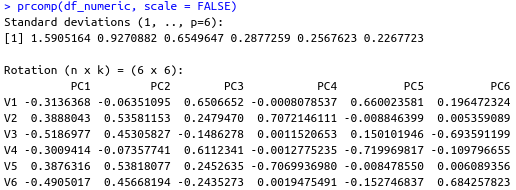
\includegraphics[width=0.80\linewidth]{../../PCA/plot/prcomp_rete-prova.png}
	\caption{Visualizzazione del calcolo della PCA tramite prcomop per il trainset di prova.}
	\label{Visualizzazione del calcolo della PCA tramite prcomop per il trainset di prova.}
\end{figure}

\begin{figure}[H]
\centering
	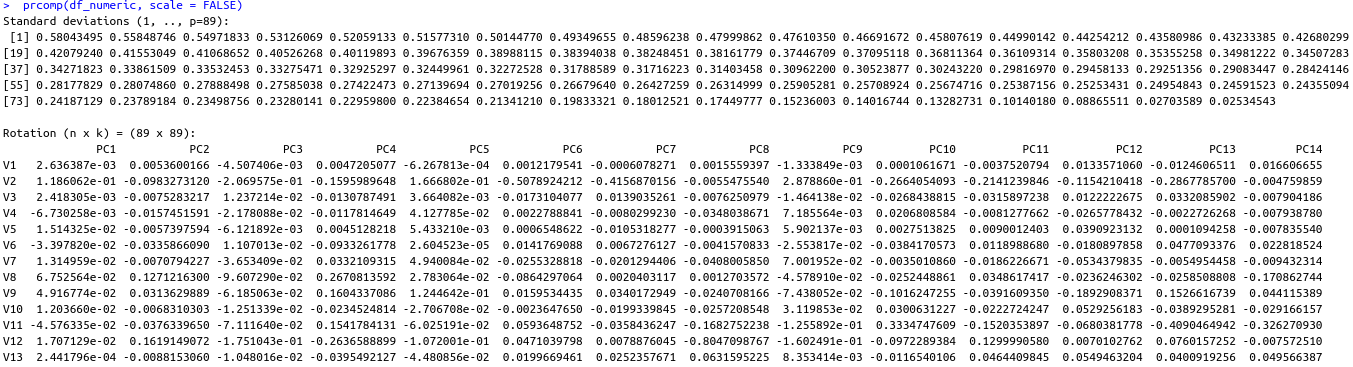
\includegraphics[width=1\linewidth]{../../PCA/plot/prcomp_rete-db.png}
	\caption{Visualizzazione del calcolo della PCA tramite prcomop per il trainset delle domande nel database.}
	\label{Visualizzazione del calcolo della PCA tramite prcomop per il trainset delle domande nel database.}
\end{figure}
\noindent

\paragraph{Osservazioni}
Osservando  esclusivamente la deviazione standard ottenuta dal trainset di prova, appare come i PC da prendere in considerazione per l'analisi sono i primi tre; inoltre  nella rotazione appare chiaro ch le valutazioni ottenute da V1 sono in relazione con V4, V3 con V6 e V2 con V5. Tuttavia queste sono solo mere osservazioni senza ancora alcuna prova matematica  completa a supporto. \\\\ Per quanto concerne il trainset delle domande nel database \`e molto difficile fare qualunque tipo di assunzione sulla natura dei dati causa la loro numerosit\`a.

\subsubsection{Calcolo degli autovettori ed individuazione di Summary}
\label{Calcolo degli autovettori ed individuazione di Summary}
\begin{figure}[H]
\centering
	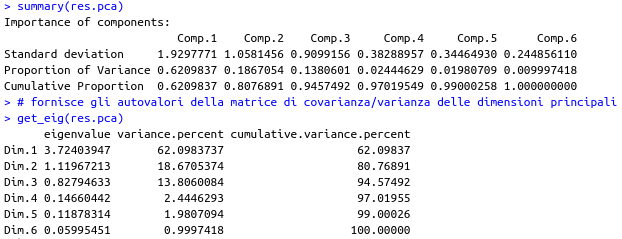
\includegraphics[width=0.80\linewidth]{../../PCA/plot/summary-autovalore_rete-prova.png}
	\caption{Visualizzazione del calcolo del metodo summary ed individuazione degli autovalori per il trainset di prova.}
	\label{Visualizzazione del calcolo del metodo summary ed individuazione degli autovalori per il trainset di prova.}
\end{figure}
\begin{figure}[H]
\centering
	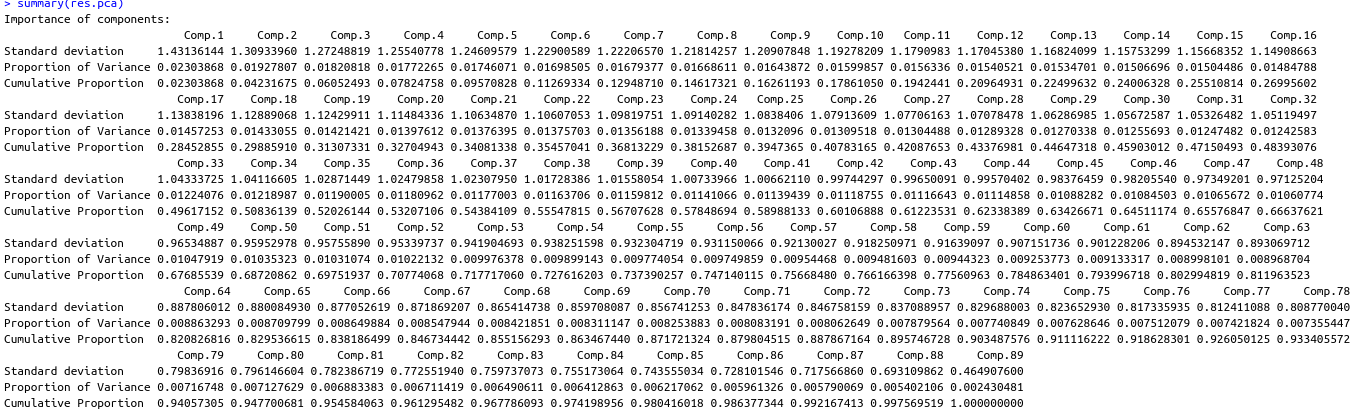
\includegraphics[width=1\linewidth]{../../PCA/plot/summary_db.png}
	\caption{Visualizzazione del calcolo del metodo summary per il trainset delle domande nel database.}
	\label{Visualizzazione del calcolo del metodo summary per il trainset delle domande nel database.}
\end{figure}
\begin{figure}[H]
\centering
	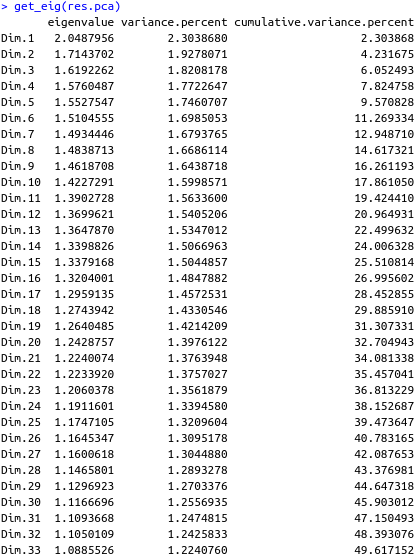
\includegraphics[width=0.60\linewidth]{../../PCA/plot/autovalori_db.png}
	\caption{Individuazione degli autovalori per il trainset delle domande nel database.}
	\label{Individuazione degli autovalori per il trainset delle domande nel database.}
\end{figure}
\paragraph{Osservazioni}
\`E essenziale per individuare il numero di componenti (PC) necessarie per effettuare un'analisi corretta basarsi sul calcolo della \textit{variance.percent} o \textit{Proportion of Variance}. A tale scopo \`e prendere le componenti principali che catturano la maggior parte di variabilti\`a dei dati.\\
Nel caso del trainset di prova basta le variabili PC1, PC2 e PC3 sono sufficienti a catturare il ~93\% della variabilit\`a presente.\\
Quanto appena descritto si pu\`o riscontrare anche graficamente, come presentato di seguito.

\begin{figure}[H]
\centering
	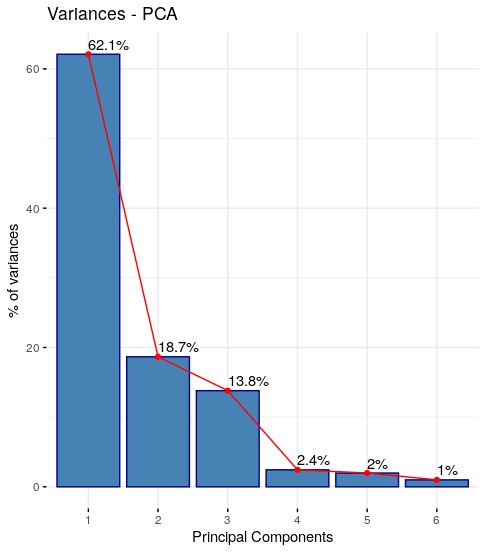
\includegraphics[width=0.60\linewidth]{../../PCA/plot/variances_rete-prova.png}
	\caption{Plot della rappresentazione grafica della varianza sui PC del trainset di prova.}
	\label{Plot della rappresentazione grafica della varianza sui PC del trainset di prova.}
\end{figure}

\begin{figure}[H]
\centering
	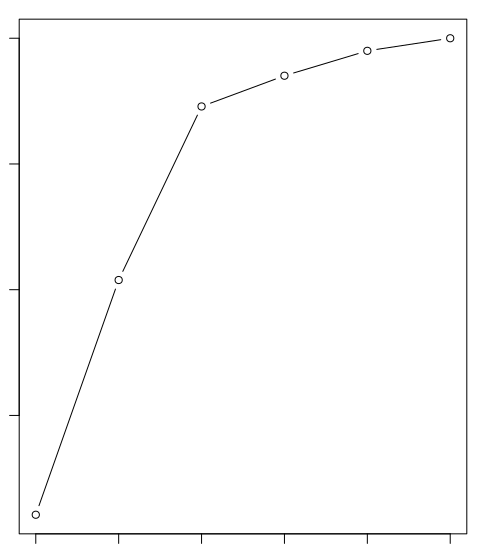
\includegraphics[width=0.60\linewidth]{../../PCA/plot/variances2_rete-prova.png}
	\caption{Plot della rappresentazione grafica della varianza sui PC del trainset di prova.}
	\label{Plot della rappresentazione grafica della varianza sui PC del trainset di prova.}
\end{figure}
\noindent
Le ultime PC4, PC5 e PC6 hanno una variabilit\`a molto bassa, trascurabile.
\begin{figure}[H]
\centering
	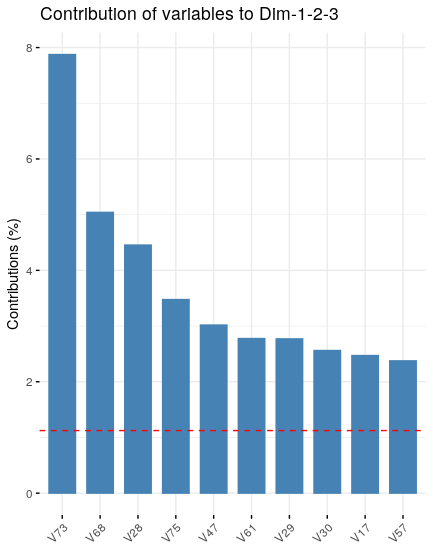
\includegraphics[width=0.60\linewidth]{../../PCA/plot/varianza-complessiva_rete-prova.png}
	\caption{Rappresentazione grafica di come la varianza si distribuisce sulle PC individuate dal modello sul trainset di prova.}
		\label{Rappresentazione grafica di come la varianza si distribuisce sulle PC individuate dal modello sul trainset di prova.}
\end{figure}
\noindent
Tuttavia per quanto riguarda le domande nel database ogni conclusione "a occhio " risulta  impossibile da effettuare sempre a causa della numerosit\`a dei dati di trainset. L'utilizzo di un analisi dei risultati per mezzo di plot \`e l'unica via percorribile.

\begin{figure}[H]
\centering
	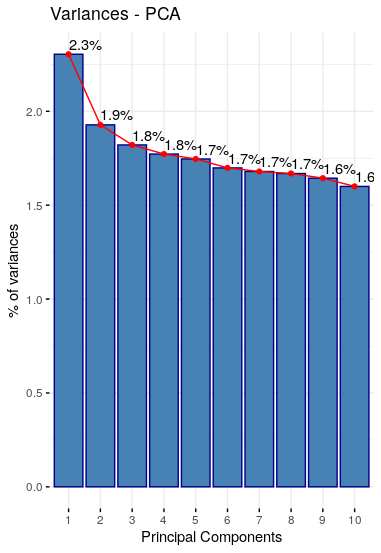
\includegraphics[width=0.60\linewidth]{../../PCA/plot/variances_rete-db.png}
	\caption{Plot della rappresentazione grafica della varianza dei primi dieci PC del trainset delle domande nel database.}
	\label{Plot della rappresentazione grafica della varianza dei primi dieci PC del trainset delle domande nel database.}
\end{figure}
\noindent
Il plot mostra esclusivamente le prime dieci componenti; tutte si presentano con una varianza molto basse. A causa di ci\`o per poter affermare quante PC sono indispensabili per una valutazione oggettiva dei dati \`e indispensabile avere una visione totalitaria di tutte variabili coinvolte nel modello.
\begin{figure}[H]
\centering
	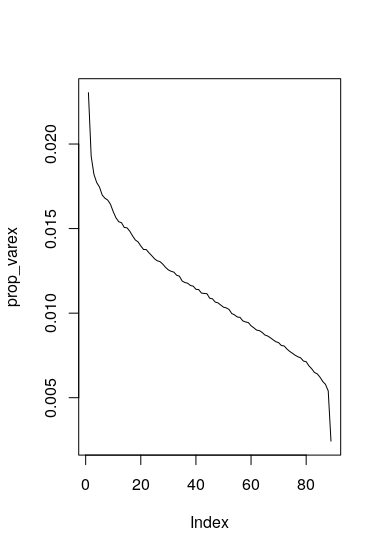
\includegraphics[width=0.60\linewidth]{../../PCA/plot/variances-ALL_rete-db.png}
	\caption{Plot della rappresentazione grafica della varianza di tutti i PC del trainset delle domande nel database.}
	\label{Plot della rappresentazione grafica della varianza di tutti i PC del trainset delle domande nel database.}
\end{figure}
\begin{figure}[H]
\centering
	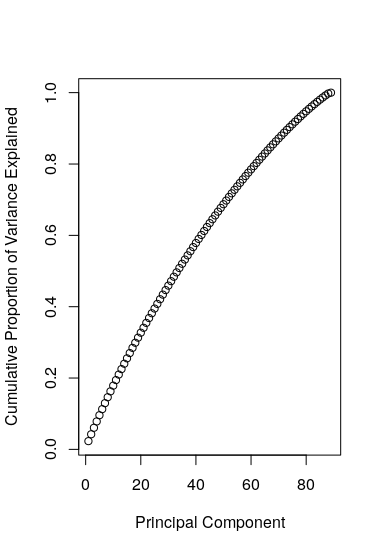
\includegraphics[width=0.60\linewidth]{../../PCA/plot/variances2-ALL_rete-db.png}
	\caption{Plot della rappresentazione grafica della varianza di tutti i PC del trainset delle domande nel database.}
	\label{Plot della rappresentazione grafica della varianza di tutti i PC del trainset delle domande nel database.}
\end{figure}
Non risulta sufficiente l'andamento dei plot per riuscire a definire il numero adeguato di componenti principali da utilizzare. In questi casi, \`e buona norma, fare riferimento a tre criteri:
\begin{itemize}
\item \textit{Quota della varianza totale}: si deve considerare un numero di CP tale che tenga conto di una percentuale sufficientemente elevata di varianza totale proporzionale al numero di variabili originarie (ovvero pi\`u \`e alto il numero di componenti del modello e pi\`u \`e accettata una percentuale minore di varianza spiegata).
\item \textit{Screen-graph}: fa uso dei plot degli autovalori in funzione al numero di CP. Gli autovalori sono decrescenti, per cui il grafico ha una buona possibilit\`a, di assumer\`a la forma di una spezzata con pendenza negativa.
\item \textit{Eigenvaue one o Regola di Kaiser}: afferma di considerare tutte ed esclusivamente le CP con autovalore maggiore di 1.
\end{itemize}
\noindent
Per soddisfare il \textit{primo criterio} \`e sufficiente fare riferimento a \textit{variance.percent} in get\_eigen o \textit{Proportion of Variance} in summary. Da questa asserzione ne consegue un quesito: quale \`e il numero di varianza accettabile avendo un numero di variabili molto elevato?.
Per effettuare una delle vie utilizzate \`e procedere al soddisfacimento del \textit{terzo criterio}. Gli autovalori di tutte le componenti coinvolte si possono vedere nella \textit{Standard deviation} risultante dalla summary. Le PC del modello, con autovalore superiore a 1, sono le PC contenute nell'intervallo 1-41.
Il \textit{secondo criterio}, invece, in questo caso specifico non \`e stato in grado di dirmi molto,  in quanto la diminuzione degli autovalori \`e graduale, senza salti evidenti.\\
In conclusione, ho considerato come una percentuale di copertura adeguata quella fornita dalla che 41 prime componenti principali.
\begin{figure}[H]
\centering
	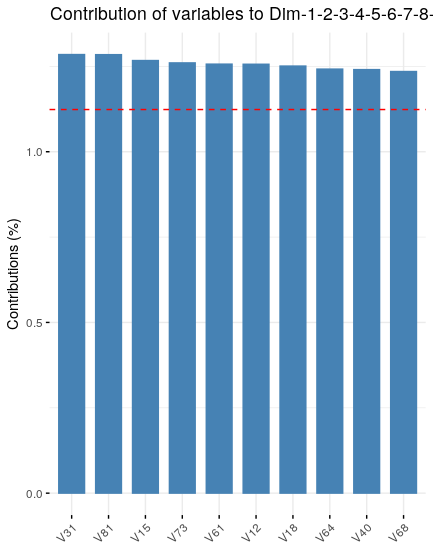
\includegraphics[width=0.60\linewidth]{../../PCA/plot/varianza-complessiva_rete-db.png}
	\caption{Rappresentazione grafica di come la varianza si distribuisce sulle PC individuate dal modello sul trainset delle domande nel database.}
	\label{Rappresentazione grafica di come la varianza si distribuisce sulle PC individuate dal modello sul trainset delle domande nel database.}
\end{figure}

\subsubsection{Calcolo degli autovettori}
\label{Calcolo degli autovettori}

\begin{figure}[H]
\centering
	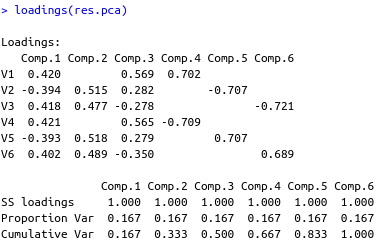
\includegraphics[width=0.60\linewidth]{../../PCA/plot/loadings_rete-prova.png}
	\caption{Autovettori del trainset di test.}
	\label{Autovettori del trainset di test.}
\end{figure}

\paragraph{Osservazioni}
L'analisi dei loadings sulle componenti principali permette di determinare il contributo delle variabili originarie al modello PC.\\
Per quanto riguarda l'analisi dei dati del trainset  la prima variabile ha valori  0.420, 0.569 e 0.702,  rispettivamente nelle componenti 1, 3 e 4 e sembra legarsi ai risultati nella variabile 4 (che riempie le medesime componenti oscillando di poco nei valori presentati), il medesimo match coinvolge le variabili 2 con 5 e 3 con 6.\\
Tali assunzioni sono molto pi\`u complesse da effettuare per  il trainset dei dati delle domande nel databas e  per fare ci\`o ho provveduto a calcolare la matrice correlazione.

\subsubsection{Calcolo della matrice di correlazione}
\label{Calcolo della matrice di correlazione}

\begin{figure}[H]
\centering
	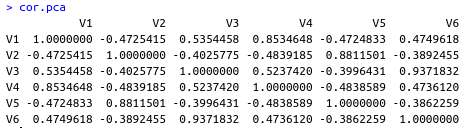
\includegraphics[width=0.60\linewidth]{../../PCA/plot/correlazione_rete-prova.png}
	\caption{Autovettori del trainset di test.}
	\label{Autovettori del trainset di test.}
\end{figure}

\begin{figure}[H]
\centering
	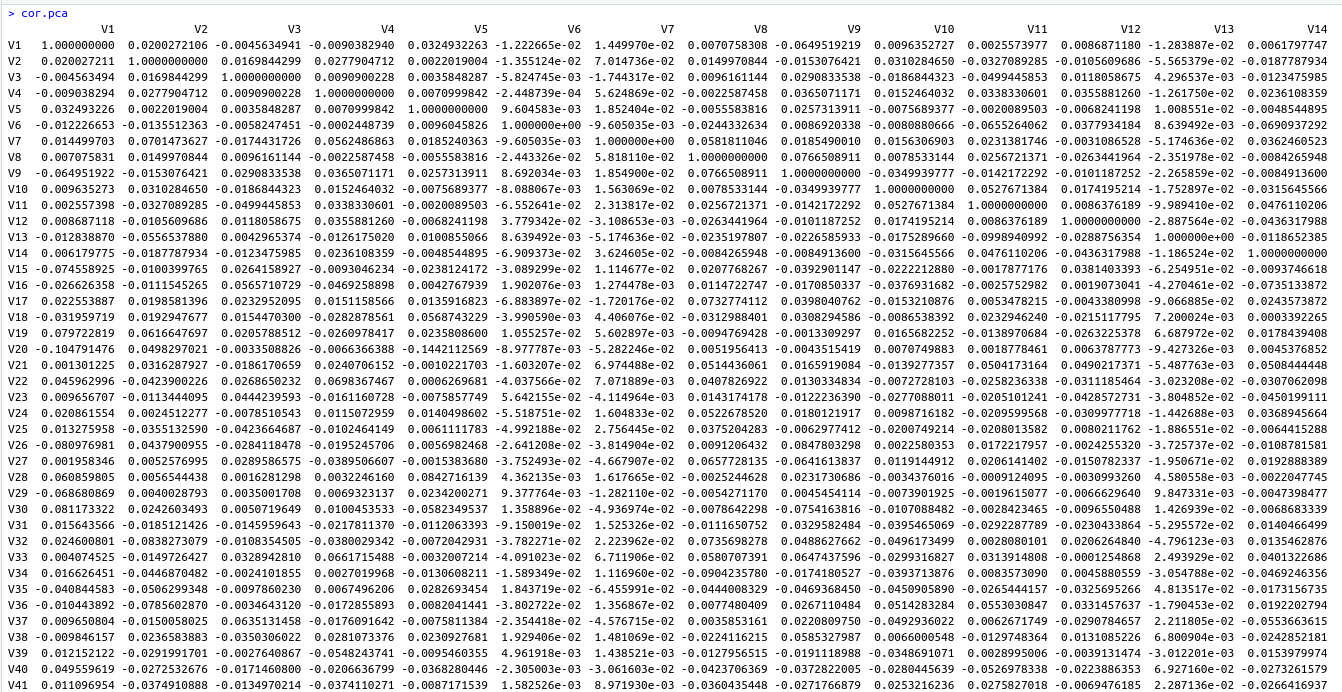
\includegraphics[width=1\linewidth]{../../PCA/plot/correlazione_rete-db.png}
	\caption{Autovettori del trainset delle domande nel database.}
	\label{Autovettori del trainset delle domande nel database.}
\end{figure}
\noindent

I CSV generati di correlazione sono i seguenti:

\begin{figure}[H]
\centering
	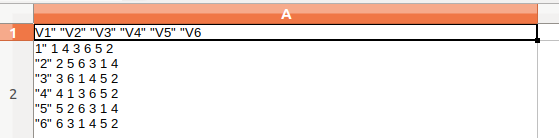
\includegraphics[width=0.60\linewidth]{../../PCA/plot/CSV_rete-prova.png}
	\caption{CSV generato a partire dalla matrice correlazione del trainset della rete di prova.}
	\label{CSV generato a partire dalla matrice correlazione del trainset della rete di prova.}
\end{figure}
\begin{figure}[H]
\centering
	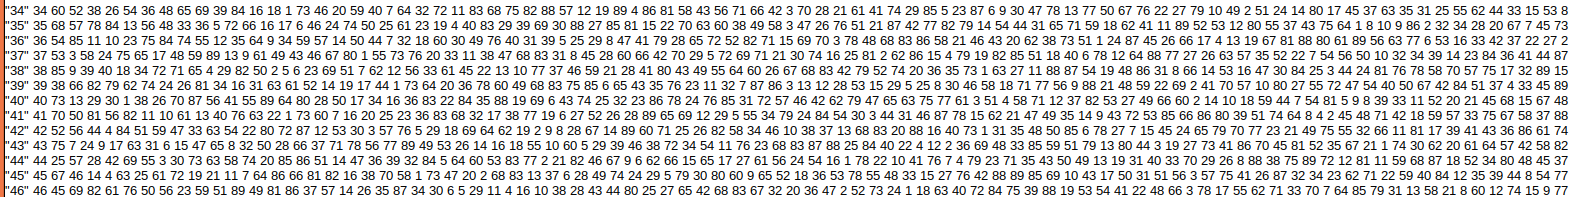
\includegraphics[width=1\linewidth]{../../PCA/plot/CSV_rete-db.png}
	\caption{CSV generato a partire dalla matrice correlazione del trainset delle domande nel database.}
	\label{CSV generato a partire dalla matrice correlazione del trainset delle domande nel database.}
\end{figure}
\noindent
I file CSV gli ho generati prendendo la matrice correlazione, che mostra il grado di correlazione di ogni componente con ogni variabile del modello, creandovi un data frame che mostra per ogni variabile quale \`e la componente a cui si collega in ordine decrescente (da  quella che si correla di pi\`u a quella che si correla di meno).\\ 
Da tale distribuzione dei dati, per il trainset di prova emerge quello che mi aspettavo. Per esempio la variabile 1 si correla con grado massimo con se stessa, successivamente con la componente 4 (che \`e la sua domanda sorella) e successivamente con le domande 3 e 6 (i suoi genitori) e alla fine con le domande 2 e 5 (nella realt\`a queste ultime due non hanno alcuna correlazione con la domanda 1). Tale ragionamento vale per tutte le altre  5 componenti, i cui risultati rimangono coerenti con le aspettative e con ci\`o che viene dichiarato nel Grafo della Conoscenza, rappresentato nella figura \ref{Grafo rappresentante le relazioni esistenti tra il set di domande di prova.} nella sezione § \ref{Test effettuati}.\\\\
Pensavo di poter effettuare il medesimo ragionamento anche per analisi dei dati del trainset del database, tuttavia questo non \`e stato possibile, a causa delle seguenti motivazioni:
\begin{itemize}
\item In primo luogo, se una variabile nella matrice correlazione \`e dichiarata in correlazione con una componente, questa poi non risulta in correlazione con la variabile;
\item Analizzando il testo delle domande, contenute nel database aziendale ho riscontrato come il modello prodotto crea relazioni strette fra domande appartenenti trivialmente a categorie diverse, (ad esempio domande che trattano relazioni con altre di serie numeriche) e meno con domande che parlano dello stesso tema.
\item Dal pot delle variabili viene mostrato come le stesse indicate come correlate risultano, invece, sparse impedendo la formazione dei cluster. Su un numero n grande di variabili  (come le 89 domande nel database) tale fenomeno verrebbe espanso impedendo a chi interpreta il modello di individuare una correlazione tra il grafico delle variabili e la matrice di correlazione.
\end{itemize}
A questo punto ho iniziato a farmi delle domande. Escludendo un mio errore di codifica (dopo aver opportunamente effettuato un accurato controllo del codice da me prodotto) e trovandomi di fronte ad una situazione dove i risultati inerenti ai dati del trainset di prova soddisfano appieno le attese
(infatti non solo le correlazioni matchano perfettamente con quanto viene indicato dal grafo della conoscenza; ma anche il plot che viene generato dalla PCA sulle variabili presenta una coerenza stretta con tali assunzioni) ho iniziato a pensare che centrasse la possibilit\`a che ha un candidato di indovinare correttamente una risposta ad una domanda.\\\\
Ho rifatto, perci\`o, tutta l'analisi su un nuovo modello, adoperando il trainset di prova generato da n input sottoposti alla probabilit\`a di indovinare. Come viene illustrato dai plots nella sezione seguente, i dati individuati dal trainset di prova puro vengono totalmente falsati quando si tiene conto di tale eventualit\`a rispetto alle aspettative imposte dal Grafo della conoscenza. 

\subsection{Conclusione dell'analisi}
\label{Conclusione dell'analisi}
In conclusione, un test con domande a triplice risposta multipla concede ad un candidato l'elevata possibilit\`a di indovinare le domande che non sa; e il modello creato dalla {P}rincipal \textbf{C}omponent \textbf{A}nalysis con i dati delle risposte alle domande nel database ne fornisce la prova.\\\\ Infatti se la possibilit\`a di indovinare fosse bassa i risultati del modello in esame ne verrebbero appena "sporcati", e invece invalidano completamente la possibilit\`a di avere un risultato attendibile e coerente con la realt\`a.\\
Le figure seguenti mostrano proprio tale fenomeno: nel caso dell'indovinato le domande con una maggiore correlazione non creano alcun cluster.

\begin{figure}[H]
\centering
	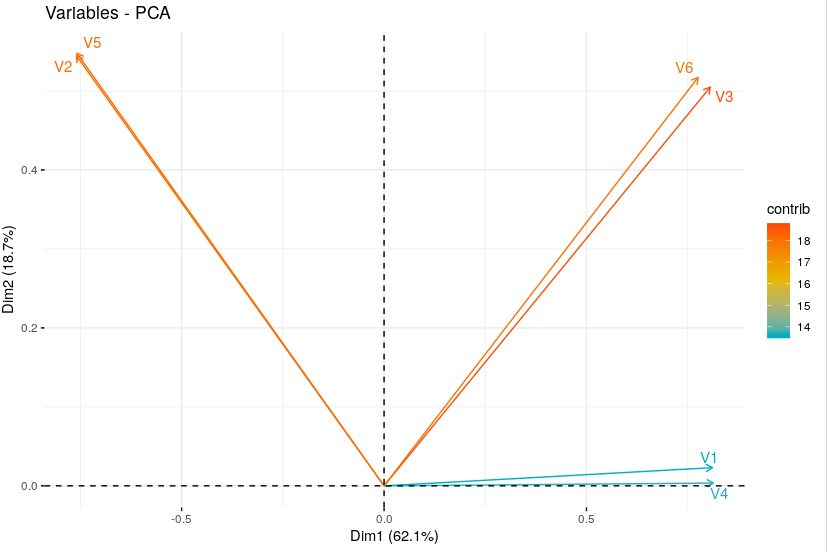
\includegraphics[width=0.80\linewidth]{../../PCA/plot/PCA.png}
	\caption{Rappresentazione per mezzo di plot di come le variabili si presentano nelle due componenti principali con il calcolo della PCA - utilizzo di trainset di prova puro sul grafo della conoscenza.}
	\label{Rappresentazione per mezzo di plot di come le variabili si presentano nelle due componenti principali con il calcolo della PCA - utilizzo di trainset di prova puro sul grafo della conoscenza.}
\end{figure}

\begin{figure}[H]
\centering
	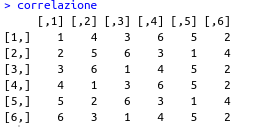
\includegraphics[width=0.60\linewidth]{../../PCA/plot/correlazione_base.png}
	\caption{Le domande in correlazione con la variabili principali in ordine decrescente sui dati di prova.}
	\label{Le domande in correlazione con la variabili principali in ordine decrescente sui dati di prova.}
\end{figure}


\begin{figure}[H]
\centering
	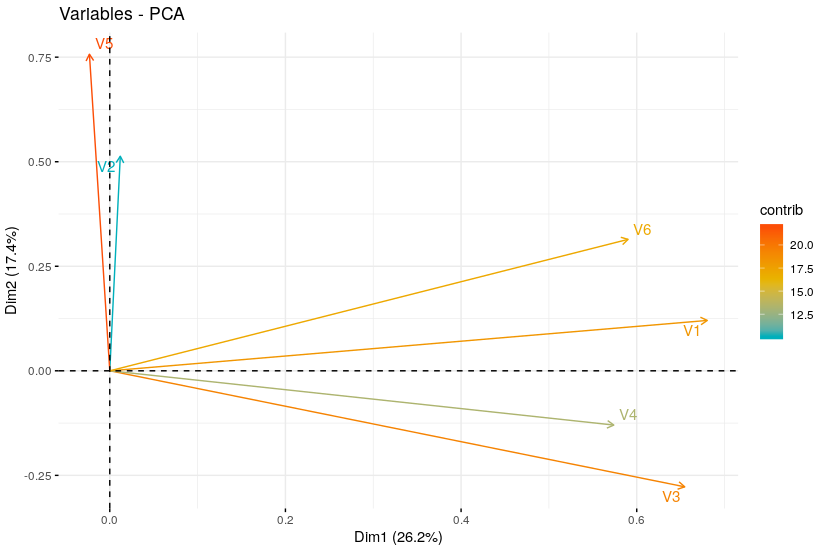
\includegraphics[width=0.80\linewidth]{../../PCA/plot/PCA-valorindovinati.png}
	\caption{Rappresentazione per mezzo di plot di come le variabili si presentano nelle due componenti principali con il calcolo della PCA - utilizzo di trainset di prova spurio con la probabilità di indovinare.}
	\label{Rappresentazione per mezzo di plot di come le variabili si presentano nelle due componenti principali con il calcolo della PCA - utilizzo di trainset di prova spurio con la probabilita di indovinare.}
\end{figure}


\begin{figure}[H]
\centering
	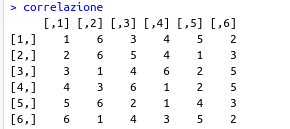
\includegraphics[width=0.60\linewidth]{../../PCA/plot/correlazione_with-probability.png}
	\caption{Le domande in correlazione con la variabili principali in ordine decrescente sui dati di prova soggetti alla probabilità di indovinare.}
	\label{Le domande in correlazione con la variabili principali in ordine decrescente sui dati di prova soggetti alla probabilita di indovinare.}
\end{figure}

\noindent L'analisi del modello ha evidenziato come il Reticolo della Conoscenza costruito  dai dati delle domande nel database, una volta costruito, risentir\`a inevitabilmente del fattore di rischio "domande indovinate". Mi aspetto, per cui, che in rapporto al contenuto delle stesse gli argomenti e la difficolt\`a  delle domande appartenenti al medesimo cluster possano non essere coincidenti.\\
L'unica possibilit\`a per continuare la costruzione del reticolo \`e rivolgere nuovamente l'attenzione alla Rete neurale e studiare i cluster possibili per mezzo delle previsioni assunte da ogni variabile sulla base della previsione standard\footnote{Vettore previsione tutto a zero}.
